% Бүлэг 3: Системийн зохиомж

\chapter{Системийн зохиомж ба дизайн}
\label{Chapter3}

\section{Системийн ерөнхий архитектур}

Энэхүү систем нь ХИЙМЭЛ ОЮУН УХААНААР ОЛОН ТӨРЛИЙН ХӨГЖИМ БА СУРГАЛТЫН ВЭБСАЙТ буюу хиймэл оюун ухаан ашиглан олон төрлийн хөгжим болон сургалтын вэбсайт хөгжүүлэх платформ юм. Систем нь дараах 5 үндсэн модулиас бүрдэнэ:

\begin{enumerate}
    \item \textbf{Хичээлийн систем (Course System)} - FL Studio хичээлүүд, явцын хяналт
    \item \textbf{AI Аудио анализ (AI Audio Analysis)} - CNN загвараар миксинг шинжилгээ, дууны чанарын үнэлгээ
    \item \textbf{Мелоди генераци (Melody Generation)} - MusicVAE загвараар аяны хувилбар үүсгэлт
    \item \textbf{RAG Чатбот (AI Assistant)} - Мэргэжлийн зөвлөгөөний систем, AI-ментор
    \item \textbf{Маркетплейс} - VST плагин, Sample Pack худалдаа
\end{enumerate}

\subsection{AI Онцлогуудын дэлгэрэнгүй тайлбар}

Энэхүү системийн гол инноваци нь хиймэл оюун ухааны гурван үндсэн функцийг нэгтгэсэн явдал юм:

\textbf{1. AI Audio Analysis (CNN)} - Хэрэглэгчийн оруулсан аудио файлыг спектрограмм болгон хувиргаж, CNN загвараар шинжлэнэ. Үр дүнд нь:
\begin{itemize}
    \item EQ зөвлөмж (дарамтамжийн тэнцвэр)
    \item Компрессор тохиргоо (динамик диапазон)
    \item Дууны чанарын үнэлгээ (100- оноо)
    \item Техникийн алдаануудын илрүүлэлт
\end{itemize}

\textbf{2. Melody Generation (MusicVAE)} - Хэрэглэгчийн MIDI файлын үндсэн дээр шинэ аяны хувилбарууд үүсгэнэ. Үр дүнд нь:
\begin{itemize}
    \item Өөр өөр жанр (pop, jazz, electronic, hip-hop)
    \item Өөр өөр хүйт (happy, sad, energetic, calm)
    \item Темпо (BPM) өөрчлөлт
    \item MIDI файл болгон экспорт
\end{itemize}

\textbf{3. AI Assistant (RAG Chatbot)} - Хэрэглэгчийн асуултанд хариулахдаа зөвхөн баталгаажсан мэдээлэл ашиглана. Үр дүнд нь:
\begin{itemize}
    \item FL Studio-ийн техникийн асуултууд
    \item Онолын мэдлэг (миксинг, мастеринг)
    \item Бүтээлч санаа (writer's block-аас гарах)
    \item Мэргэжлийн зөвлөгөө
\end{itemize}

Систем нь \textbf{Multi-layer Architecture} буюу олон давхаргат архитектурын дагуу зохион байгуулагдсан:

\begin{itemize}
    \item \textbf{Client Layer (Frontend)}: Next.js React application
    \item \textbf{API Layer}: Supabase Edge Functions
    \item \textbf{Data Layer}: PostgreSQL database
    \item \textbf{AI Layer}: CNN, MusicVAE, LLM services
    \item \textbf{Storage Layer}: Supabase Storage (audio files)
\end{itemize}

Хүснэгт \ref{tab:SystemComponents}-т системийн үндсэн бүрэлдэхүүн хэсгүүд болон тэдгээрийн техникийн тодорхойлолтыг үзүүлэв.

\begin{table}[htbp]
\centering
\caption{Системийн үндсэн бүрэлдэхүүн хэсгүүд}
\label{tab:SystemComponents}
\begin{tabular}{|l|p{6cm}|p{5cm}|}
\hline
\textbf{Бүрэлдэхүүн} & \textbf{Технологи} & \textbf{Үүрэг} \\
\hline
Frontend & Next.js 14, React, TypeScript & Хэрэглэгчийн интерфейс \\
\hline
Backend API & Supabase Edge Functions & HTTP хүсэлт боловсруулалт \\
\hline
Database & PostgreSQL & Өгөгдлийн хадгалалт \\
\hline
Vector DB & Pinecone & RAG хайлтын мэдээлэл \\
\hline
AI Models & TensorFlow, PyTorch & CNN, MusicVAE, LLM \\
\hline
File Storage & AWS S3 / Supabase Storage & Аудио файл хадгалалт \\
\hline
Authentication & Supabase Auth & Хэрэглэгч баталгаажуулалт \\
\hline
\end{tabular}
\end{table}

\subsection{Архитектурын диаграм}

Зураг \ref{fig:Architecture}-т системийн ерөнхий архитектурыг харуулав.

\begin{figure}[htbp]
    \centering
    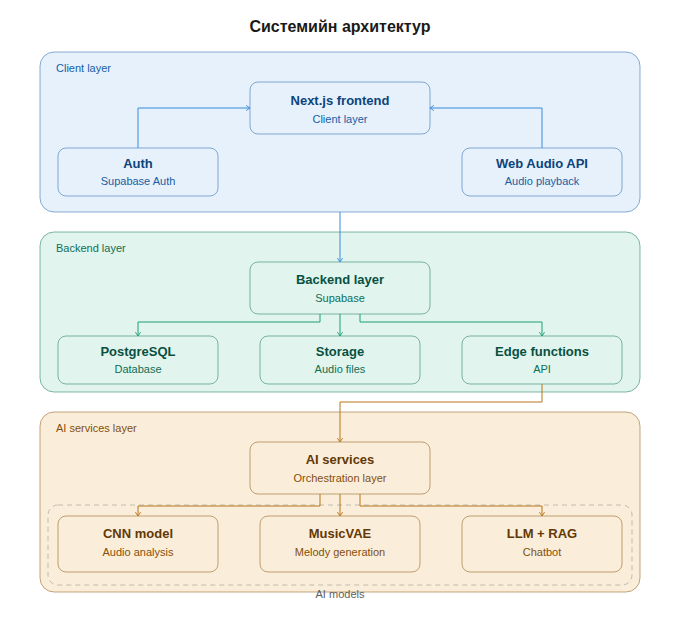
\includegraphics[width=0.9\textwidth]{Diagrams/01_system_architecture}
    \caption[Системийн ерөнхий архитектур]{Системийн ерөнхий архитектур}
    \label{fig:Architecture}
\end{figure}

\section{Юзкейс (Use Case) диаграм}

Зураг \ref{fig:UseCaseAI}-т системийн юзкейс диаграмыг харуулав.

\begin{figure}[htbp]
    \centering
    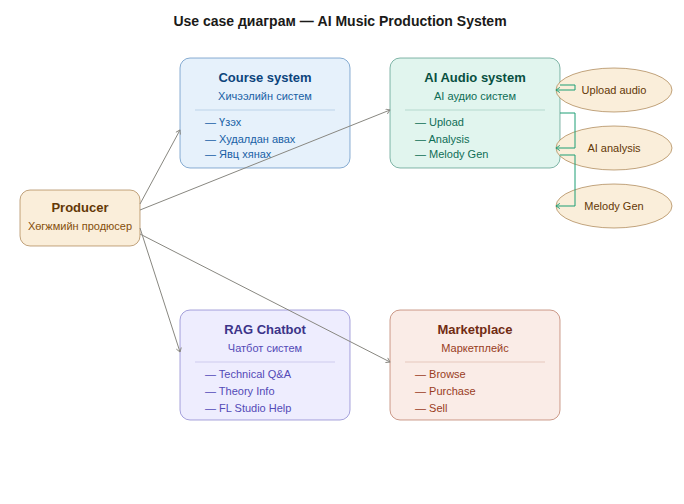
\includegraphics[width=0.85\textwidth]{Diagrams/02_use_case_diagram}
    \caption[Системийн Юзкейс диаграм]{Системийн Юзкейс диаграм}
    \label{fig:UseCaseAI}
\end{figure}

Системийн үндсэн оролцогч нь \textbf{Producer (Хөгжмийн продюсер)} бөгөөд дараах үйлдлүүдийг хийж болно:

\subsection{Хичээлийн систем юзкейсууд}
\begin{itemize}
    \item Хичээлүүд үзэх (View Courses)
    \item Хичээл худалдан авах (Purchase Course)
    \item Видео үзэж сурах (Watch Lessons)
    \item Сурах явц хянах (Track Progress)
    \item Дуусгасан хичээл тэмдэглэх (Mark Completed)
\end{itemize}

\subsection{AI Аудио систем юзкейсууд}
\begin{itemize}
    \item Аудио файл байршуулах (Upload Audio)
    \item AI анализ хийлгэх (AI Analysis)
    \item EQ зөвлөмж авах (Get EQ Recommendations)
    \item Компрессор тохиргоо авах (Get Compression Settings)
    \item Мелоди генераци хийлгэх (Generate Melody Variations)
\end{itemize}

\subsection{Чатбот юзкейсууд}
\begin{itemize}
    \item Техникийн асуулт асуух (Ask Technical Question)
    \item Онолын мэдээлэл авах (Get Theory Information)
    \item FL Studio-ийн тухай асуух (FL Studio Q\&A)
\end{itemize}

\subsection{Маркетплейс юзкейсууд}
\begin{itemize}
    \item Зүйлс үзэх (Browse Items)
    \item Зүйл худалдан авах (Purchase Item)
    \item Өөрийн зүйл зарах (Sell Item)
    \item Файл татаж авах (Download File)
\end{itemize}

\section{Өгөгдлийн урсгалын диаграм}

Зураг \ref{fig:DataFlow}-т системийн өгөгдлийн урсгалыг харуулав. Энэ нь хэрэглэгчийн аудио файлаас эхлэн AI анализ, үр дүнг хүртэлх бүх үйл явцыг илэрхийлнэ.

\begin{figure}[htbp]
    \centering
    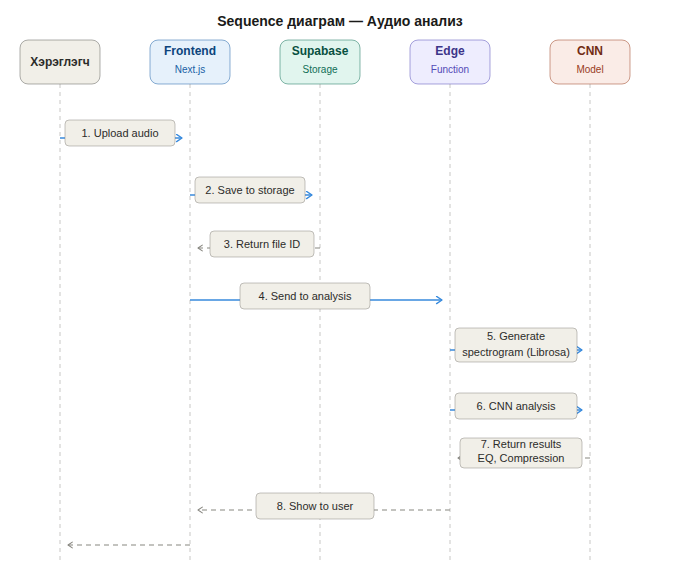
\includegraphics[width=0.85\textwidth]{Diagrams/03_sequence_audio_analysis}
    \caption[Өгөгдлийн урсгалын диаграм]{Өгөгдлийн урсгалын диаграм}
    \label{fig:DataFlow}
\end{figure}

\subsection{Өгөгдлийн урсгалын тайлбар}
Хүснэгт \ref{tab:DataFlowExplanation}-т өгөгдлийн урсгалын үе шатуудыг дэлгэрэнгүй тайлбарлав.

\begin{table}[htbp]
centering
\caption{Өгөгдлийн урсгалын үе шатууд}
\label{tab:DataFlowExplanation}
\begin{tabular}{|l|p{10cm}|}
\hline
\textbf{Үе шат} & \textbf{Тайлбар} \\
\hline
1. Файл оруулалт & Хэрэглэгч аудио файл (.wav, .mp3) оруулна \\
\hline
2. Хадгалалт & Файл Supabase Storage-д хадгалагдана \\
\hline
3. STFT хувиргалт & Аудио спектрограм болгон хувиргана \\
\hline
4. CNN инференс & Спектрограммыг CNN загвараар шинжлэнэ \\
\hline
5. Үр дүн боловсруулалт & EQ, компрессор зөвлөмж үүсгэнэ \\
\hline
6. Хариу буцаах & Үр дүнг хэрэглэгчид харуулна \\
\hline
\end{tabular}
\end{table}

\section{Дарааллын (Sequence) диаграмууд}

\subsection{Аудио анализын дарааллын диаграм}

Аудио анализ үйл явцын дараалал (Зураг \ref{fig:SeqAudioAnalysis}):

\begin{enumerate}
    \item Хэрэглэгч аудио файл байршуулна
    \item Frontend файлыг Supabase Storage-д хадгална
    \item Edge Function файлыг авч, spectrogram үүсгэнэ
    \item CNN загвар спектрограмм дээр анализ хийнэ
    \item Үр дүн (EQ зөвлөмж, чанар үнэлгээ) буцаагдана
    \item Хэрэглэгчид график хэлбэрээр харуулна
\end{enumerate}

\begin{figure}[htbp]
    \centering
    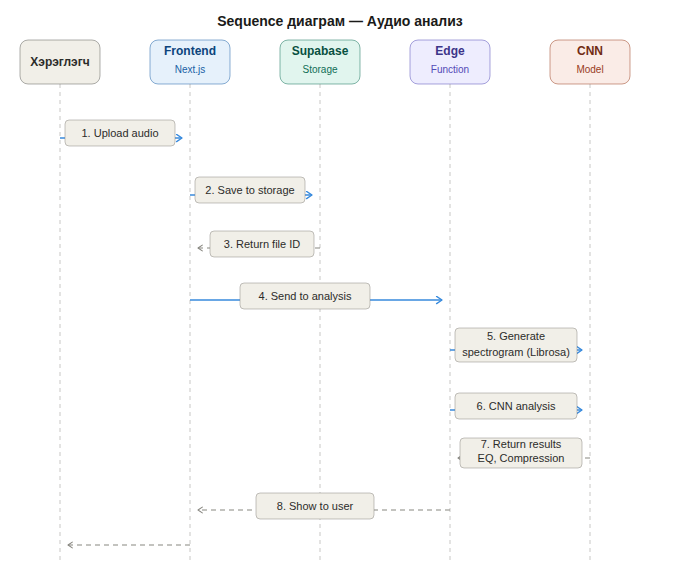
\includegraphics[width=0.9\textwidth]{Diagrams/03_sequence_audio_analysis}
    \caption[Аудио анализын дарааллын диаграм]{Аудио анализын дарааллын диаграм}
    \label{fig:SeqAudioAnalysis}
\end{figure}

\subsection{RAG Чатбот дарааллын диаграм}

Чатбот ажиллах дараалал (Зураг \ref{fig:SeqRAGChatbot}):

\begin{enumerate}
    \item Хэрэглэгч асуулт илгээнэ
    \item Query embedding үүсгэнэ
    \item Vector database-д similarity search хийнэ
    \item Олсон контекстийг LLM-ээд илгээнэ
    \item LLM хариулт үүсгэнэ
    \item Хариултыг хэрэглэгчид харуулна
\end{enumerate}

\begin{figure}[htbp]
    \centering
    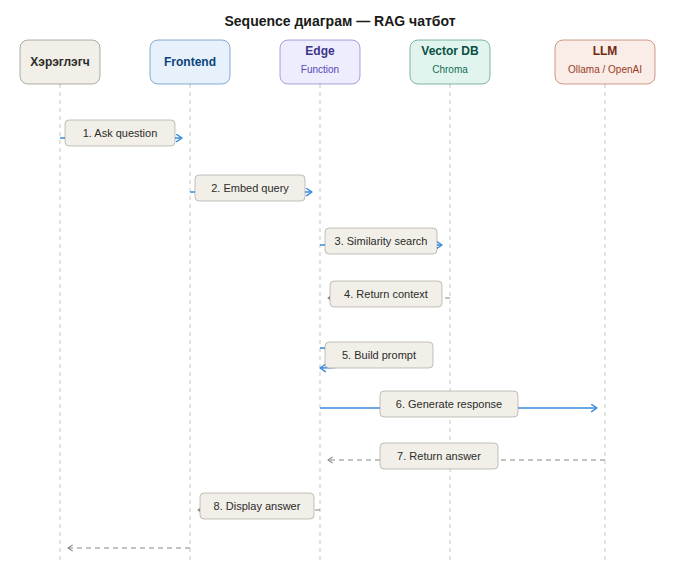
\includegraphics[width=0.9\textwidth]{Diagrams/04_sequence_rag_chatbot}
    \caption[RAG Чатбот дарааллын диаграм]{RAG Чатбот дарааллын диаграм}
    \label{fig:SeqRAGChatbot}
\end{figure}

\section{Өгөгдлийн сангийн диаграм}

\subsection{Өгөгдлийн ерөнхий схем}

Өгөгдлийн сангийн хүснэгтүүд хоорондоо дараах холбоосоор холбогдоно:
\begin{itemize}
    \item \textbf{auth.users} $\rightarrow$ \textbf{profiles}: 1:1 холбоос
    \item \textbf{profiles} $\rightarrow$ \textbf{purchased\_courses}: 1:N холбоос
    \item \textbf{profiles} $\rightarrow$ \textbf{audio\_files}: 1:N холбоос
    \item \textbf{audio\_files} $\rightarrow$ \textbf{mixing\_analysis}: 1:N холбоос
    \item \textbf{profiles} $\rightarrow$ \textbf{chat\_messages}: 1:N холбоос
\end{itemize}

Өгөгдлийн сангийн ерөнхий схемийг доорх хүснэгтэд үзүүлэв:

\begin{table}[htbp]
\centering
\caption{Өгөгдлийн сангийн хүснэгтүүд}
\label{tab:DatabaseTables}
\begin{tabular}{|l|p{10cm}|}
\hline
Хүснэгт & Тайлбар \\
\hline
profiles & Хэрэглэгчийн профайл \\
\hline
purchased\_courses & Худалдан авсан хичээлүүд \\
\hline
audio\_files & Байршуулсан аудио файлууд \\
\hline
mixing\_analysis & AI анализын үр дүн \\
\hline
melody\_variations & Мелодийн хувилбарууд \\
\hline
knowledge\_base & Мэдлэгийн сан (RAG) \\
\hline
chat\_messages & Чатбот мессежүүд \\
\hline
marketplace\_items & Борлуулалтад гаргасан зүйлс \\
\hline
payments & Төлбөрийн мэдээлэл \\
\hline
\end{tabular}
\end{table}

Системийн өгөгдлийн сан нь PostgreSQL дээр суурилсан бөгөөд дараах хүснэгтүүдээс бүрдэнэ:

\subsection{Хэрэглэгч болон профайл}
\begin{itemize}
    \item \textbf{auth.users} - Supabase authentication
    \item \textbf{profiles} - Хэрэглэгчийн профайл (id, full\_name, avatar\_url, bio)
\end{itemize}

\subsection{Хичээлийн систем}
\begin{itemize}
    \item \textbf{purchased\_courses} - Худалдан авсан хичээлүүд
    \item \textbf{completed\_lessons} - Дуусгасан хичээлүүд
    \item \textbf{course\_progress} - Сурах явцын хувь
\end{itemize}

\subsection{AI систем}
\begin{itemize}
    \item \textbf{audio\_files} - Байршуулсан аудио файлууд
    \item \textbf{mixing\_analysis} - AI анализын үр дүн
    \item \textbf{melody\_variations} - Үүсгэсэн мелодийн хувилбарууд
    \item \textbf{knowledge\_base} - Мэдлэгийн сан (RAG)
    \item \textbf{chat\_messages} - Чатбот мессежүүд
\end{itemize}

\subsection{Маркетплейс}
\begin{itemize}
    \item \textbf{marketplace\_items} - Борлуулалтад гаргасан зүйлс
    \item \textbf{payments} - Төлбөрийн мэдээлэл
\end{itemize}

\section{Төлөвийн диаграм}

Хэрэглэгч хичээл үзэх явцад дараах төлөвүүдээр шилждэг (Зураг \ref{fig:StateCourse}):
\begin{itemize}
    \item \textbf{Нэвтрээгүй} → Нэвтрэх
    \item \textbf{Нэвтрээгүй} → Бүртгүүлэх
    \item \textbf{Нэвтрээгүй} → Үнэгүй хичээл үзэх
    \item \textbf{Нэвтрэсэн} → Хичээл сонгох
    \item \textbf{Нэвтрэсэн} → Хичээл үзэх
    \item \textbf{Үзэж байгаа} → Дуусгасан
\end{itemize}

\begin{figure}[htbp]
    \centering
    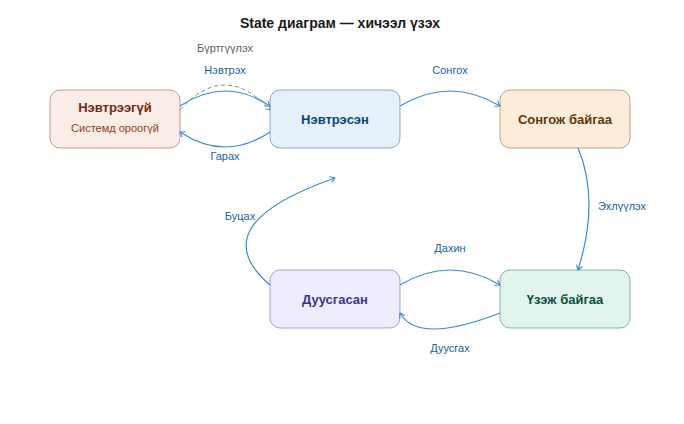
\includegraphics[width=0.8\textwidth]{Diagrams/05_state_diagram}
    \caption[Хичээл үзэх төлөвийн диаграм]{Хичээл үзэх төлөвийн диаграм}
    \label{fig:StateCourse}
\end{figure}

\section{График диаграмууд}

\subsection{Технологийн стек}

Системийн технологийн бүтэц:

\begin{itemize}
    \item \textbf{Frontend}: Next.js 14, TypeScript, TailwindCSS
    \item \textbf{Backend}: Supabase (PostgreSQL, Edge Functions, Storage)
    \item \textbf{AI}: TensorFlow/Keras (CNN), Magenta (MusicVAE), LangChain (RAG)
    \item \textbf{Authentication}: Supabase Auth (JWT)
    \item \textbf{Deployment}: Vercel (Frontend), Supabase Cloud (Backend)
\end{itemize}

Төслийн хугацаа (Зураг \ref{fig:Timeline}):

\begin{enumerate}
    \item \textbf{Анализ ба шаардлага} (1-2 долоо хоног)
    \item \textbf{Зохиомж} (2-3 долоо хоног)
    \item \textbf{Хэрэгжүүлэлт} (6-8 долоо хоног)
    \item \textbf{Тест ба сайжруулалт} (2-3 долоо хоног)
\end{enumerate}

\begin{figure}[htbp]
    \centering
    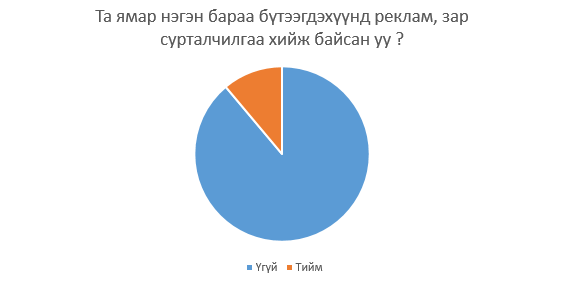
\includegraphics[scale=0.6]{Chart/Chart1}
    \caption[Төслийн хугацаа]{Төслийн хугацаа}
    \label{fig:Timeline}
\end{figure}

Хэрэглэгчийн сурах зам:

\begin{enumerate}
    \item Бүртгүүлэх / Нэвтрэх
    \item Хичээл сонгох
    \item Хичээл худалдан авах (шаардлагатай бол)
    \item Видео үзэх
    \item Дасгал хийх
    \item AI тусламж авах
\end{enumerate}

AI системийн ажиллах дараалал:

\begin{enumerate}
    \item Аудио файл байршуулах
    \item Spectrogram үүсгэх (Librosa)
    \item CNN загвараар анализ хийх
    \item EQ/Compression зөвлөмж гаргах
    \item Үр дүн харуулах
\end{enumerate}

\section{Хэрэглэгчийн интерфейс дизайн}

Дашбоард хуудасны \textbf{Frontend implementation} - `Frontend/src/app/dashboard/page.tsx`:

\begin{lstlisting}[language=JavaScript]
// Хэрэглэгчийн дашбоард
export default function DashboardPage() {
  const [user, setUser] = useState(null);
  
  return (
    <div className="min-h-screen bg-[#0A0A0F]">
      <h1>Тавтай морил</h1>
      <p>FL Studio-н хичээлүүд</p>
      <div className="grid">
        {courses.map((course) => (
          <Link href={`/courses/${course.slug}`}>
            {course.title}
          </Link>
        ))}
      </div>
    </div>
  );
}
\end{lstlisting}

\section{Бүлгийн дүгнэлт}

Энэ бүлгээр системийн зохиомжийг нарийвчлан гаргасан байна. Юзкейс диаграм нь хэрэглэгчдийн үйл ажиллагааг тодорхойлсон бол, дарааллын диаграмууд нь системийн дотоод үйл ажиллагааг харуулна. Өгөгдлийн сангийн схем нь өмнөх бүлэгт тодорхойлсон функциональ шаардлагуудтай тохирч байгаа төдийгүй ирээдүйн өргөтгөлд бэлтгэсэн архитектуртай болно.

Дараагийн бүлэгт хэрэгжүүлэлтийн нарийвчлол болон ашигласан технологиудыг авч үзэх болно.
